\begin{exercise}{2016/17 1}
    Βρείτε δύο διαφορετικά παραδείγματα συστημάτων στο επίπεδο με σημείο
    ισορροπίας στο \( (0, 0) \) το οποίο ενώ έχει γειτονιά \( N_{\epsilon}(0) \)
    τέτοια ώστε \( x \in N_{\epsilon}(0) \Rightarrow \lim_{t \to \infty} \phi(x,
    t) = 0 \), δεν είναι ευσταθές κατά \tl{Lyapunov}. Εξηγήστε γιατί τέτοια
    παραδείγματα είναι κατ᾽ ανάγκην μη-γραμμικά.
\end{exercise}
\begin{solution}{2016/17 1}
    Το σημείο \( \bar{x} \) είναι ευσταθές σημείο ισορροπίας αν για κάθε
    γειτονιά \( U \) του \( \bar{x} \), υπάρχει γειτονιά \( U_1 \) του
    \( \bar{x} \) τέτοια ώστε κάθε λύση \( x(t) \) με \( x(0) \) στο \( U_1 \),
    να υπάρχει και να ορίζεται στο \( U \) για κάθε \( t > 0 \). Αν το \( U_1 \)
    μπορεί να επιλεχθεί έχοντας τις ιδιότητες που περιγράφηκαν και ακόμα ισχύει
    \( \lim_{t \to \infty} x(t) = \bar{x} \), τότε το \( \bar{x} \) είναι
    ασυμπτωτικά ευσταθές. Στην άσκηση μας δίνεται ότι η λύση είναι
    συγκλίνουσα στο \( 0 \) και μας δίνεται μία γειτονιά του \( 0 \) που
    οι λύσεις είναι συγκλίνουσες. Αυτό όμως δεν προϋποθέτει ότι το σημείο
    είναι ευσταθές στη γενική περίπτωση, καθώς τίποτα δε μας διασφαλίζει ότι
    για κάθε \( U \), που θα φράζει τη \( x(t) \), θα μπορούμε να βρούμε λύσεις
    που ξεκινούν στη \( N_{\epsilon}(0) \) και θα παραμένουν εντός του συνόλου
    \( U \). Συνεπώς, μπορούμε κάλλιστα να έχουμε μία συμπεριφορά όπως
    αυτή που απεικονίζεται στο σχήμα~\ref{fig:ex1_unstable_convergent}.
    \begin{figure}[h]
        \centering
        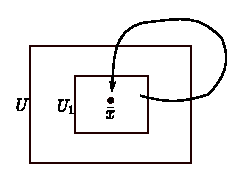
\includegraphics[width=0.4\textwidth]{figures/ex1_unstable_convergent.eps}
        \caption{\gr{Ασταθές, συγκλίνων σημείο.}}
        \label{fig:ex1_unstable_convergent}
    \end{figure}

    Ένα παράδειγμα που παρουσιάζει αυτή τη συγκλίνουσα αλλά ασταθή συμπεριφορά
    είναι το παρακάτω.
    \begin{align*}
        \dot{x}_1 &= x_1^2 - x_2^2 \\
        \dot{x}_2 &= 2x_1^2x_2^2.
    \end{align*}
    Το σημείο ισορροπίας του συστήματος είναι το \( (0, 0) \). Κάθε τροχιά του
    συστήματος τείνει στην αρχή των αξόνων καθώς \( t \to \infty \), εκτός από
    τις τροχιές που ξεκινούν στον άξονα \( x_1 \), οι οποίες παραμένουν εκεί για
    κάθε χρόνο. Στο σχήμα~\ref{fig:ex1_unstable_convergent_example} βλέπουμε το
    διάγραμμα του διανυσματικού πεδίου για το παράδειγμά μας.
    \begin{figure}[h]
        \centering
        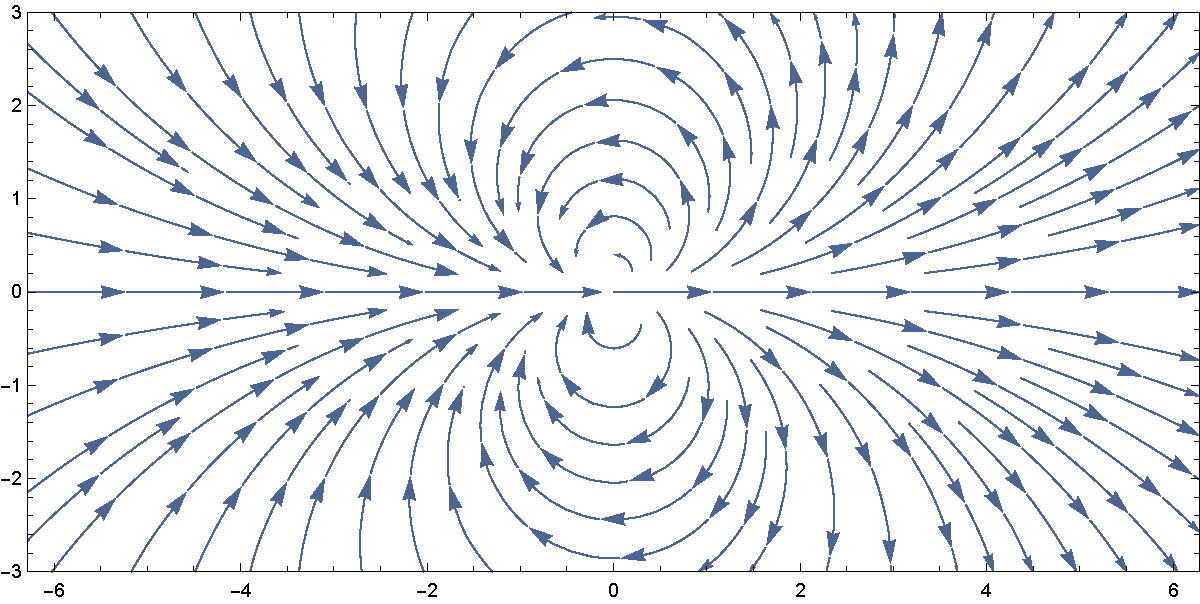
\includegraphics[width=0.8\textwidth]{figures/ex1_unstableConvergentExample.pdf}
        \caption{\gr{Παράδειγμα ασταθούς, συγκλίνουν σημείου.}}
        \label{fig:ex1_unstable_convergent_example}
    \end{figure}

    Τέτοια παραδείγματα είναι κατ᾽ ανάγκην μη-γραμμικά. Η ευστάθεια ενός
    γραμμικού συστήματος της μορφής
    \begin{equation*}
        \dot{x}(t) = Ax(t), \quad x(0) = x_0,
    \end{equation*}
    εξαρτάται αποκλειστικά και μόνο από τη φασματική δομή του πίνακα \( A \).
    Επίσης, το σύστημα έχει τη γνωστή λύση
    \begin{equation*}
        x(t) = e^{At}x_0.
    \end{equation*}
    Επομένως, ο μόνος τρόπος ώστε η παραπάνω να ικανοποιεί το \( \lim_{t \to
    \infty} \phi(x, t) \) είναι οι ιδιοτιμές του πίνακα \( A \) να έχουν
    αρνητικό πραγματικό μέρος. Αυτό εύκολα φαίνεται αν πάρουμε τη μορφή
    \tl{Jordan} του πίνακα \( A \), έτσι στη διαγώνιο θα έχουμε τις ιδιοτιμές
    και το ζητούμενο όριο θα ικανοποιείται μόνο όταν είναι αρνητικές. Αυτό
    σημαίνει ότι, για τα γραμμικά συστήματα αν ικανοποιείται το όριο τότε αυτό
    σημαίνει και ασυμπτωτική ευστάθεια.
\end{solution}
